%% ID: bead_on_wire
%% TITLE: Bead on a wire
%% TYPE: question
%% QUESTIONTYPE:  numerical
%% CONCEPTS: forces, friction, newtoni, newtonii
%% VIDEOS: 
%% LEVEL: 5
%% TOPIC: mechanics/statics
%% ORDER: 7

\begin{problem}[A1989MsQ6l] %Friction, parametric equations
{\question{A rough wire is bent into shape such that it obeys the parametric equations $x=3p^2$ and $y=2p^3$ for $p\ge 0$. The wire is then placed in a vertical plane such that the \vari{y}-axis is vertical and the \vari{x}-axis horizontal. A bead of mass \vari{m} is then threaded onto the wire. The bead is then pulled in the direction of increasing \vari{x} by a force \vari{F} of magnitude \vari{3mg}. The coefficient of friction \vari{\mu} between the wire and the bead is \vari{\frac{1}{2}}, find the set of points at which the bead can remain in equilibrium.}
{\textit{Used with permission From UCLES, A Level Maths, Syllabus C, June 1989, Special Paper, Question 6.}}
{\answer{Since our wire approaches but never reaches \quantity{90}{$^\circ$}, limiting equilibrium is never reached again for values of \vari{x} greater than 3. This is our set of equilibrium positions. }
Let's first get the two parametric equations into a Cartesian form so we can visualise the shape of the wire:

\begin{eqnarray*}
\text{Let:} x^3 = (3p^2)^3 \text{ and } y^2 = (2p^3)^2 \\
\text{Equate $p^6$:} \frac{y^2}{4} = \frac{x^3}{27} \\
y = \frac{2\sqrt{3}}{9}x^{\frac{3}{2}} 
\end{eqnarray*}

 We can see a representation of this in Figure \ref{fig:Statics_parametric_wire_1}. The $3mg$ pulling force is added for visualisation purposes only.
 
 \begin{figure}[h]
	\centering
	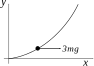
\includegraphics[width=0.35\textwidth]{Statics_parametric_wire_1}
	\caption{}	
	\label{fig:Statics_parametric_wire_1}
\end{figure}

Now we should consider all the forces acting on the bead. We will have two situations, one where the bead is in limiting equilibrium with the frictional force, $F_r$ working to prevent the bead being dragged upwards ($a$), and another limiting equilibrium situation where in the bead will be high up the curve, with Friction working to prevent the bead slipping down ($b$). We can also add the normal contact force, $R$, and the weight of the bead, $mg$, to the diagram. See Figure \ref{fig:Statics_parametric_wire_2}:

 \begin{figure}[h]
	\centering
	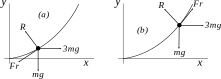
\includegraphics[width=0.7\textwidth]{Statics_parametric_wire_2}
	\caption{}	
	\label{fig:Statics_parametric_wire_2}
\end{figure}

First consider situation ($a$). We want to be working in terms of an angle, $\theta$. The easiest thing to do will be to call the angle above the horizontal $\theta$, as can be seen in Figure \ref{fig:Statics_parametric_wire_3}, and then resolve vertically and horizontally, as well as use $F_r = \mu R$ to give us an equation in $\theta$. 

 \begin{figure}[h]
	\centering
	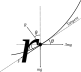
\includegraphics[width=0.4\textwidth]{Statics_parametric_wire_3}
	\caption{}	
	\label{fig:Statics_parametric_wire_3}
\end{figure}

\begin{align*} \intertext{Vertically:} Rcos{(\theta)} &= mg + F_r\sin{(\theta)} \\
\intertext{Horizontally:} 3mg&=R\sin{(\theta)} +F_r\cos{(\theta)} \\
\intertext{Remove $mg$:} 3(R\cos{(\theta)} - F_r\cos{(\theta)}) &= R\sin{(\theta)} + F_r\cos{(\theta)} \\
\intertext{Since $R = 2 F_r$ (friction):} 6F_r\cos{(\theta)} - 3F_r\sin{(\theta)} &= 2F_r \sin{(\theta)} +F_r \cos{(\theta)} \\
5F_r\cos{(\theta)} &= 5F_r\sin{(\theta)} \\
\tan{(\theta)} &= 1 \end{align*}

This is remarkably convenient since $\tan{(\theta)}$ is also our gradient function ($\frac{opposite}{adjacent} = \frac{rise}{tread} = gradient$). So simply find $\frac{dy}{dx}$ and equate to $\tan{(\theta)} = 1$ which will give us a value of $x$ for which the system is in limiting equilibrium:

\begin{align*}y &= \frac{2\sqrt{3}}{9}x^{\frac{3}{2}} \\
\\ \frac{dy}{dx} &= \frac{\sqrt{3}}{3}x^{\frac{1}{2}} = 1 \\
\\ \sqrt{(3x)} &= 3 \\
\\x = 3 \textrm{ hence } y &= \frac{2\sqrt{3}}{9}\times (3)^{\frac{3}{2}} = 2 \\
\intertext{Point of limiting equilibrium =} (3,2) \end{align*}

This is saying that for values of $x$ greater than $3$, the bead will not slip UP the wire. However, there is another possibility to consider (assuming we can place the bead along the wire at any point we like): slipping DOWN the wire, previously denoted as situation ($b$). The method is identical, just with the frictional force, $F_r$ working in the opposite direction along the tangent:

\begin{eqnarray*} 
\text{Vertically:} F_r\sin{(\theta)} + Rcos{(\theta)} &= mg\\
\text{Horizontally:} R\sin{(\theta)} &=3mg+F_r\cos{(\theta)} \\
\text{Remove $mg$ and $R$:} 2F_r\sin{(\theta)} &= 3(F_r\sin{(\theta)} +2F_r\cos{(\theta)} ) +F_r\cos{(\theta)}  \\
-F_r\sin{(\theta)} &= 7F_r\cos{(\theta)}  \\
\tan{(\theta)} &= -7 \end{align*}

This is a slight problem in terms of our original visualisation, and it is saying that limiting equilibrium is only reached when $\theta$ is negative or greater than $90^\circ$. Hence, since our wire approaches but never reaches $90^\circ$, we need not worry about situation ($b$) - limiting equilibrium is never reached again for values of $x$ greater than 3. This is our set of equilibrium positions. 


}
\end{problem}